\documentclass[conference,compsoc, twocolumn]{IEEEtran}
\ifCLASSOPTIONcompsoc
  \usepackage[nocompress]{cite}
\else
  \usepackage{cite}
\fi
\ifCLASSINFOpdf
\else
\fi
  \usepackage{amsmath} 
  \usepackage{array}
  \usepackage{fixltx2e}
  \usepackage{stfloats}
  \usepackage{url}
  \usepackage{graphicx}
  \usepackage{here}
\hyphenation{data-base}

\begin{document}

\title{Baseball-AI\\ Winning Rate Computing}

\author{\IEEEauthorblockN{Ji Am Chung\IEEEauthorrefmark{1},
Young Jae Byun\IEEEauthorrefmark{2},
Seung Myeon Park\IEEEauthorrefmark{3}, 
Jun Jeon\IEEEauthorrefmark{4}}
\IEEEauthorblockA{\IEEEauthorrefmark{1}Department of Information System\\
Hanyang University\\
Seoul, Korea\\ Email: hummernk@gmail.com}
\IEEEauthorblockA{\IEEEauthorrefmark{2}Department of Information System\\
Hanyang University\\
Seoul, Korea\\ Email: qusdudwowo@gmail.com}
\IEEEauthorblockA{\IEEEauthorrefmark{3}Department of Information System\\
Hanyang University\\
Seoul, Korea\\ Email: antimoto@nate.com}
\IEEEauthorblockA{\IEEEauthorrefmark{4}Department of Information System\\
Hanyang University\\
Seoul, Korea\\ Email: jeonjun2@gmail.com}}

\maketitle

\begin{abstract}
\quad Today baseball is becoming more and more popular and getting new fans. Those who just have put their first step into baseball - find it hard to follow the rules and to understand the changes in the situation. Unlike our baseball league KBO, MLB already has many meaningful methods for in-game analyzing with real time statistics. So we are going to adopt those ideas into KBO league. Winning Probability Added, which is also known as WPA, is one of good factors which allows easy understanding of the situation and the impacts that pitcher or batter makes each time. Our project aims to show ‘Winning Rate’ and ‘WPA factor’ in real-time, with the algorithm that fits KBO situation.
\end{abstract}
% no keywords


\section{Introduction}
% no \IEEEPARstart
\quad Baseball, even though the myriad scandals, attracts more and more fans and is becoming more nationwide sports. There is a major  problem that, though baseball fans are inflowing, it’s hard for beginners to understand the rules and catch situation of the match. Though baseball is much more a number-oriented sport than any others such as soccer or basketball, the classical stats do not fully reflect the match stream and evaluate the value of the players properly. However, in MLB, a lot of sabermetricians have already quantified vague situations and values in numerical way, and KBO tends to follow it. (i.e Babip, OPS, etc..). Korean baseball websites nowadays use the same WPA algorithm which had been used in earlier days of MLB, so the differences between two leagues are not considered. We wanted to solve this problem by creating our own WPA algorithm based on KBO, which not only calculates the stats suitable for KBO, but also analyzes winning possibilities of each team and the impacts each players make. We also focus on helping beginners to understand baseball.
\quad We will make KBO winning rate DB and we are going to put that into our program. The program  represents ongoing situation of the match and each team’s winning possibilities simultaneously. Also, by showing quantified stats such as batters’ WPA or pitchers’ WAR , it shows how much powerful the player is(or has been) throughout the game, seasons or his entire career. Whether baseball match is underway or not, the program will show player rank categorized by players, teams, or positions according to user’s request.
\quad It is not just ‘Baseball statistic calculator’, but also somewhat like websites such as Statiz or KBReport. The software indicates different types of statistical analysis, and shows them in visualized ways. We thought that current WPA algorithm used in korean web sites does not fit korean baseball situation. That is why we have started this project.

This project is composed of 4 steps.
\begin{enumerate}
\item Crawl the data of  last 10 seasons of KBO from baseball statistics websites. 
\item Compute the data to make some statistics.
\item Apply the statistics to WPA algorithm.
\item Real-time data capturing and showing the winning rate and WPA.
\end{enumerate}
% You must have at least 2 lines in the paragraph with the drop letter
% (should never be an issue)

\hfill May 2, 2016



\section{Requirements}



\subsection{Data Handling}


\subsubsection{Crawling}
\begin{itemize}
\item Get every single raw data of  KBO from baseball webpage to construct the root database.
\item Crawiling source : http://www.koreabaseball.com
\end{itemize}

\subsubsection{Capturing}
\begin{itemize}
\item Get real-time data when the match is underway.
\end{itemize}

\subsubsection{Real-Time Mirroring}
\begin{itemize}
\item Program should immediately renew the database according to the result of the match.
\end{itemize}

\subsubsection{Computing}
\begin{itemize}
\item Calculate the numerical data to make some meaningful statistics.
\item Every single data has different weight.
e.g.)\ Hits at 1st inning have different value from those at 9th.
\item Calculate numerical values including WPA.
\end{itemize}

\subsubsection{Data Storage}
\begin{itemize}
\item Save every single stats data.
\item Divide players  into two tables. One table is for players who is in active service, the other for retired.
\item Table for players who is in active service needs to be updated constantly, and the other table doesn’t.
\item User who wants to conceal  the program from screen can do that by clicking ‘window minimization’ button.
\end{itemize}

\subsection{Function}


\subsubsection{EXCEL Compatibility}
\begin{itemize}
\item User can export datas of specific player or stats  to MS Excel files.
\item User can import fixed form of MS Excel file of specific game result to compute changes of KBO algorithm winning rate shown as image file which can also exported as jpeg, gif, png, or bmp.
\item User can import fixed form of MS Excel file of specific league(fantasy or amatuer) data to compute WAR stats. This data can be exported as EXCEL file.
\end{itemize}

\subsubsection{On-Board Posting(abandoned)}
\begin{itemize}
\item Someone who wants to post any idea or thoughts can share what they have.
\item Make another Q\&A board so as to hel beginners solve their curiosity.
\end{itemize}

\subsubsection{Board Log-in \& Sign-out(abandoned)}
\begin{itemize}
\item Log-in to or Sign-out from Board.
\item User who logged-in the board can upload their post or reply to other users’
\end{itemize}

\subsubsection{Stats Visualization}
\begin{itemize}
\item Show current state of game in a table.
\item Show current winning average of each team 
\item Show current WPA stats of players
\item Show player's photograph
\end{itemize}

\subsection{User Interface}


\subsubsection{Window Minimization \& Window Maximization}
\begin{itemize}
\item User who wants to see the program widely can do that by clicking ‘window maximization’ button
\end{itemize}

\subsubsection{Program Turn On \& Turn Off}
\begin{itemize}
\item User can turn on the program by clicking ‘desktop icon’ 
\item If user try to power on the program even if that is already turned on, terminate existing program and launch the program again
\item User can turn off the program by clicking ‘x button’ at the top-right corner of the program
\end{itemize}

\subsubsection{Mouse Click Event}
\begin{itemize}
\item Provide user with three options [To Home, Window Minimization, Termination] when user right-click any area within program.
\end{itemize}

\subsubsection{Player Stat Pop-Up}
\begin{itemize}
\item When user clicks certain player, program shows his profile by generating a new pop-up
\item If player is a pitcher, pop up list of the first string who has not been on the match yet
\item If player is taking the field, pop up his profile as batter
\item Pitcher pop-up profile stats list : ERA(Earned Run Average) for applicable season, WPA, WAR, WHIP for last 5 matches, (K\/BB 9), hyperlink connected to NAVER article about him
\item Batter pop-up profile stats list : BA(Batting Average), WAR, WPA, OPS for last 5 matches, BABIP for applicable season, \quad hyperlink connected to NAVER article about him
\item The number of pop-up cannot be over two
\end{itemize}

\subsubsection{Player Ranking}
\begin{itemize}
\item Sort players by team, position, date and game with WPA stats
\end{itemize}

\subsubsection{Data Searching}
\begin{itemize}
\item Searching option constitutes of match schedule, player and stats and player
\item If option ‘match schedule’ is chosen, program shows match schedule as a calendar
\item If user click one of date, there are three cases. First one is ‘past match’, so program shows match log. Second one is ‘on-going match’, so program directs user to the match. And the last one is ‘coming match’, so program shows every details of  the match including players, referees, park,  appointed first thrower, weather forecast 
\item If option ‘player and stat’ is chosen, program shows the applicable stats by entire players, team, position, monthly separately.
\item If option ‘player’ is chosen, program shows every single stat of applicable player
\end{itemize}

\subsubsection{Get Information real-time}
\begin{itemize}
\item User can choose the way one gets some information(pop-up or push window)
\item Pop-up is a kind of window, so when user have it on the screen, one cannot click main program
\item Information could be as follows
\item Agreed Decision : User can get information about agreed decision and its details
\item Cancellation in case of rain : User can get information when the match is cancelled in case of rain by getting a pop-up or push window
\item Player Substitutution : In case of substituting player, User can get information why the player was substituted with other, and information about that ‘other’ player
\item When option is ‘pop-up’, user can have additional function which is ‘Multi-View’.  By doing so, user can watch several matches simultaneously
\item If there have multiple pop-ups, eliminate pop-up windows sequentially after checking them
\end{itemize}

\subsubsection{Error}
\begin{itemize}
\item Error alert
\end{itemize}



\section{Development Environment}



\subsection{Choice of Software Development Platform}


\subsubsection{Which platform and why? (e.g.\ , Windows, Linux, Web, or etc.\ )}
\begin{itemize}
\item We adopted Windows, because there are some merit when we choose Windows. First of all, the percentage of all Windows user is almost 85\%. Since we want to emphasize on majority, we chose Windows. Second, because of encoding compatibility. For more convenience, it’s much better to share encoding method in OS, web server, database.
\end{itemize}

\subsubsection{Which programming language and why?}
\begin{itemize}
\item  We used both python and Java. At first we used only python 2.7 to crawl html source, to parse tag data and manipulate date with python DB driver. But pyhon 2.7 had problem of unicode encoding. 
Because the web site that we wanted to crawl was encoded with 'utf-8', but python doesn't support it.
So we have to think another IDE. Two candidates was python 3.5, who support 'utf-8' and Java with a friendly programming language. With a contempletation, we decided that crawl, parsing and DB manipulation by using python 3.5 and the others, GUI, etc. by Java. That's because we had not enough time to learn a new Jave crawling, parsing code, but only to have time to transplant python 2.7 code into python 3.5. And we were not sure whether python 3.5 is an effective tool for GUI making, so we adopted Java IDE Netbeans which support easy GUI method.
\end{itemize}

\subsubsection{Provide a cost estimation for your built.\\
 (including any purchase of software/hardware)}
\begin{itemize}
\item human labor - 0 \\
Our group constitute of four members who all do this group term project voluntarily. So human labor cost is zero.
\item software cost - 0  \\
Our group will make program with open source API,  which costs zero for academic purpose.
\item hardware cost - 0  \\
Our group uses our existing laptop to simulate or implement our program. There is no need to buy other hardware. 
\end{itemize}

\subsubsection{Provide clear information of your development environment.\\
(e.g., version of software, OS version, your computer resources)}
\begin{itemize}
\item OS \\
Windows 10 pro(10586.218 build)
\item Language Set \\
Korean
\item Computer Mode l\\
MSI GT60
\item Processor \\
Intel(R) Core(TM) i7-3600QM	CPU @ 2.4GHz
\item Main Memory \\
8GB RAM
\item Internet Connection \\
IPTIME WiFi
\end{itemize}


\subsection{Software in use}


\subsubsection{Any existing software or algorithm in use? (doing a similar task as
your proposal; provide a proper reference if there is any)}
\begin{itemize}
\item There is no similar software computing WPA, after Tom Tango introduced concepted of WPA. But, there is several websites or spreadsheet providing 
each statement winning rate. For MLB, there is a site called 'The Book'. It is made by Tom Tango who designed many good index including WPA. 'Statiz', 
'KBReport' are sites providing many baseball stats for KBO.
\end{itemize}
\\
Statiz
\begin{figure}[H]
\centering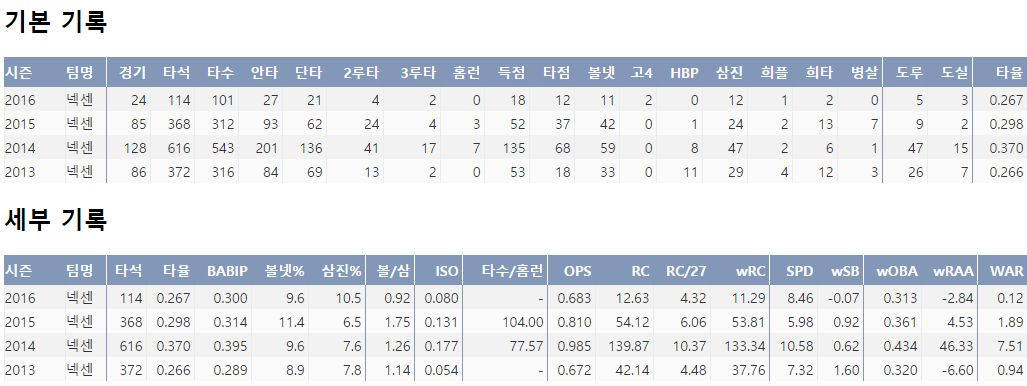
\includegraphics[width=6cm]{Statiz}     
\caption{Statiz}
\end{figure}
\\
\\
\\

KBReport
\begin{figure}[H]
\centering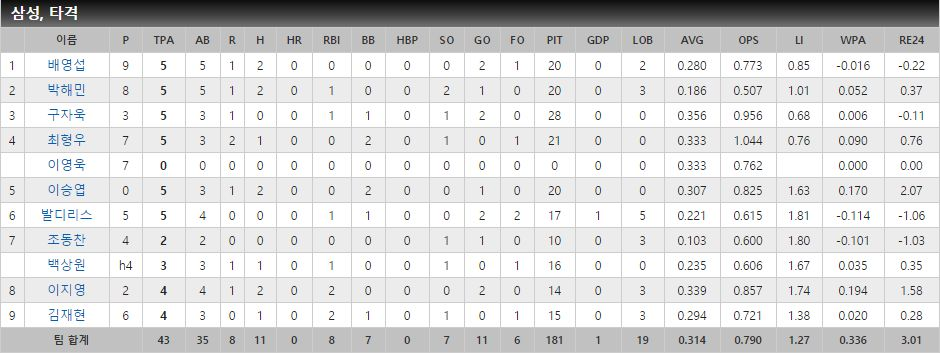
\includegraphics[width=6cm]{KBReport}    
\caption{KBReport}
\end{figure}

TheBook
\begin{figure}[H]
\centering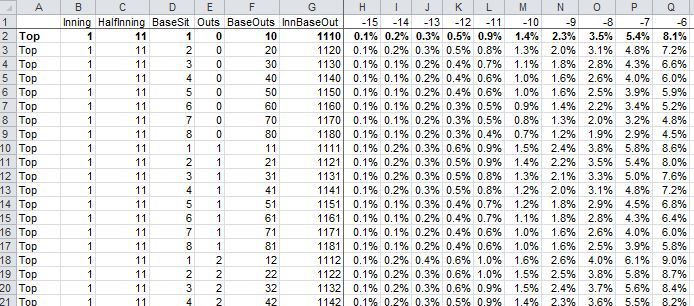
\includegraphics[width=6cm]{TheBook}
\caption{TheBook}
\end{figure}




\subsection{Task distribution (If you want, you can provide this
later at the next phase - design)}

\begin{itemize}
\item Which member is responsible for what?
\end{itemize}
\begin{center}
\begin{tabular}{1|1|1} \hline
Roles				& name 					& task description\  	\\ \hline
User     				& Jun Jeon				& test some modules 	\\ \hline
Customer      			&  Seung Myun Park		& return feedback		\\ \hline
Software developer 	&  Y	oung Jae Byun		& develop modules	\\ \hline
Development manager&  Ji Am Chung			& organize architecture\\ \hline
\end{tabular}
\end{center}
\\


\section{Specification}

\subsection{Data Handling}

\subsubsection{Crawling}
\begin{figure}[H]
\centering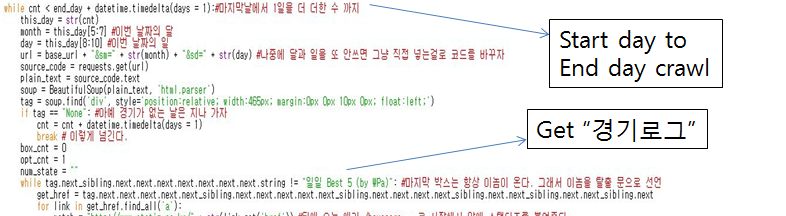
\includegraphics[width=6cm]{CrawlingSource}
\caption{Crawling source}
\end{figure}
\begin{figure}[H]
\centering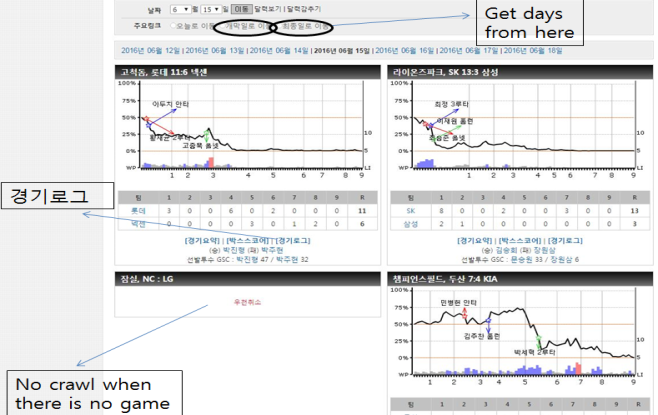
\includegraphics[width=6cm]{ParsingSource}
\caption{Parsing source}
\end{figure}

\begin{itemize}
\item Users can set the start date and end day that includes matches they want to crawl.
\item The crawler gets data from baseball webpage to construct the database.
\item Data means game box score which contains every statement in actual game.
\item It cralws form the homepage: \\
http://www.koreabaseball.com/Schedule/Game/BoxScore.aspxleagueId=n1&seriesId=n2&gameId=yyyymmddtlt2x&gyear=yyyy\\
n1 of leagueId and n2 of SeriesID are arbitrary integer number, yyyymmddt1t2x of gameId is year, month, day, team1, team2, I digit ordinal number, yyyy of gyear is year.
\end{itemize}

\begin{figure}[H]
\centering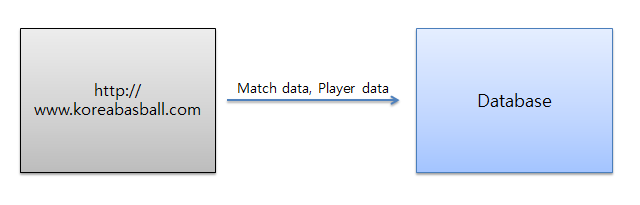
\includegraphics[width=6cm]{requirement1-a}
\caption{crawling}
\end{figure}

\subsubsection{Capturing}

\begin{itemize}
\item Get real-time data when match is underway.
\end{itemize}

\begin{figure}[H]
\centering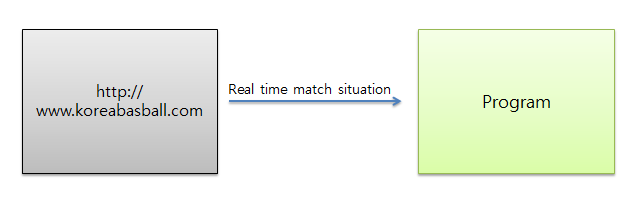
\includegraphics[width=6cm]{requirement1-b}
\caption{capturing}
\end{figure}

\subsubsection{Real-Time Mirroring}

\begin{itemize}
\item Program should immediately renew the database according to the result of the match.
\end{itemize}

\begin{figure}[H]
\centering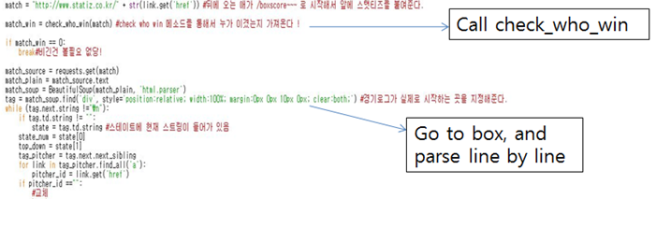
\includegraphics[width=6cm]{CrawlingRealtimeCode}
\caption{Crawling Real-time Code}
\end{figure}
\begin{figure}[H]
\centering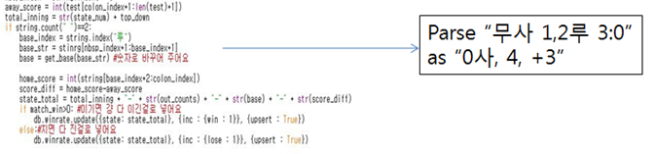
\includegraphics[width=6cm]{ParsingRealtimeCode}
\caption{Parsing Real-time Code}
\end{figure}
\begin{figure}[H]
\centering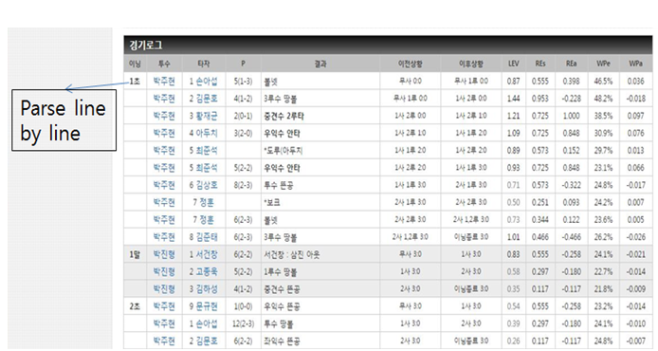
\includegraphics[width=6cm]{CrawlingRealtimeSource}
\caption{Crawling Real-time Source}
\end{figure}
\begin{itemize}
\item After the data is crawled, crawler checks who is winning at the specific time, ans parse the data line-by line and puts the value into the program.
\end{itemize}
\begin{itemize}
\item After the data is put on the program, it shows current situation of the match real-time.
\end{itemize}
\begin{figure}[H]
\centering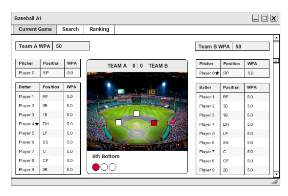
\includegraphics[width=6cm]{RealtimeGUI}
\caption{Real-time GUI}
\end{figure}
\begin{itemize}
\item If the base is on with a batter, it filled with color ‘red’ and if the base is not on, it filled with color ‘white’
\end{itemize}
\begin{figure}[H]
\centering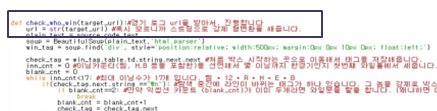
\includegraphics[width=6cm]{CrawlingWhoWonCode1}
\caption{Crawling who won code1}
\end{figure}
\begin{figure}[H]
\centering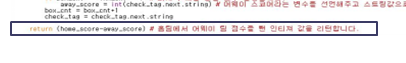
\includegraphics[width=6cm]{CrawlingWhoWonCode2}
\caption{Crawling who won code2}
\end{figure}
\begin{figure}[H]
\centering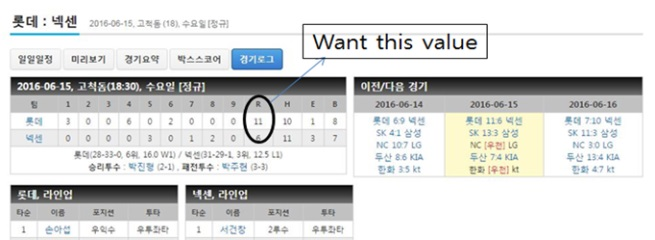
\includegraphics[width=6cm]{CrawlingWhoWonSource}
\caption{Crawling who won that game source}
\end{figure}
\begin{itemize}
\item When the match ends, real-time crawler gets the information of which team won the game, and ends with setting the value 1 to won team and 0 to lost team.
\end{itemize}




\begin{figure}[H]
\centering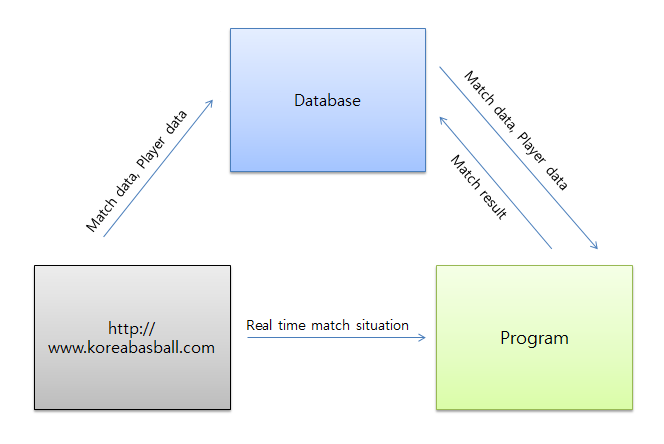
\includegraphics[width=6cm]{requirement1-c}
\caption{real-time mirroring}
\end{figure}

\subsubsection{Computing}

\begin{itemize}
\item We can calculate Winning rate as follows. 
\begin{equation} \label{eq:winrate} Winrate = \frac{All Matches\cap Statement\cap Win}{All Matches\cap Statement} \end{equation}
\end{itemize}



\subsubsection{Data Storage}
\begin{itemize}
\item Save every single stats data.
\item Divide players  into two tables. One table is for players who is in active service, the other for retired.
\item Table for players who is in active service needs to be updated constantly, and the other table doesn’t.
\end{itemize}



\subsection{Functions}

\subsubsection{EXCEL Compatibilty}

\begin{itemize}
\item User can export data in the program that she/he wants.
\item playerorstats.xlsl is an example of excel file daeling with datas of specific player or stats.
\item gameres.jpeg is an example of image file that can be exported from a fixed form of MS Excel file of specific game result, which computes changes of KBO 
algorithm winning rate.

\begin{figure}[H]
\centering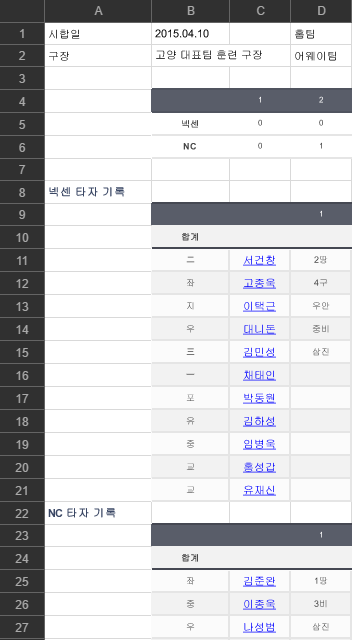
\includegraphics[width=6cm]{input}
\caption{excel input file}
\end{figure}

\begin{figure}[H]
\centering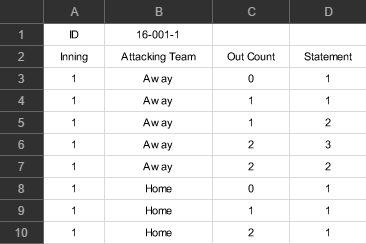
\includegraphics[width=6cm]{output}
\caption{excel output file}
\end{figure}
\item leaguedata.xlsl is an example of fixed form of MS Excel file of specific league(fantasy or amatuer) data to compute WAR stats.
\end{itemize}

\subsubsection{On-Board Posting(X)}
\begin{itemize}
\item Someone who wants to post any idea or thoughts can share their idea.
\item Make another Q&A board so as to help beginners solve their curiosity.
\end{itemize}

\subsubsection{Board Log-in \& Sign-out(X)}
\begin{itemize}
\item Log-in to or Sign-out from Board.
\item User who logged-in the board can upload their post or reply to other post.
\end{itemize}

\subsubsection{Stats Visualization}
\begin{itemize}
\item cur\_state.myd is an example of mysql data file showing current state of game in a table form.
\item By Generating a new pop-up, program can show user current winning average of each team.
\item By Generating a new pop-up, program can show user current WPA stats of players.
\item By Generating a new pop-up, program can show player's photograph.
\end{itemize}



\subsection{User Interface}


\subsubsection{Window Minimization & Window Maximization}
\begin{itemize}
\item Window default size : 960*540
\item User who wants to conceal the program from the screen can do that by clicking ‘window minimization’ button.
\item User who wants to see the program widely can do that by clicking ‘window maximization’ button.
\item User can turn off the program by clicking ‘x button’ at the top-right corner of  the program.
\end{itemize}

\begin{figure}[H]
\centering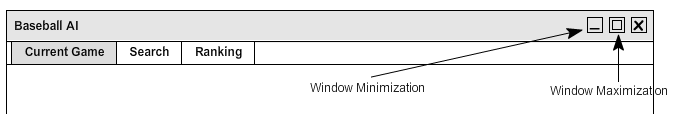
\includegraphics[width=6cm]{WindowMaxMin}
\caption{Windows Minim.\&Maxim.}
\end{figure}

\subsubsection{Program Turn On \& Turn Off}
\begin{itemize}
\item User can turn on the program by clicking ‘desktop icon’.
\end{itemize}

\begin{figure}[H]
\centering\includegraphics[width=6cm]{icon}
\caption{Program Turn On}
\end{figure}

\begin{itemize}
\item If user try to power on the program even if that is already turned on, terminate existing program and launch program again.
\end{itemize}

\begin{itemize}
\item User can turn off the program by clicking ‘x button’ at the top-right corner of  the program.
\end{itemize}

\begin{figure}[H]
\centering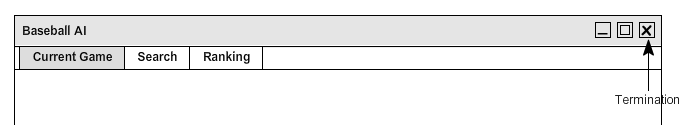
\includegraphics[width=6cm]{WindowTerminate}
\caption{Program Turn Off}
\end{figure}

\subsubsection{Mouse Click Event}
\begin{itemize}
\item Provide user with three options [To Home, Window Minimization, Termination] when user right-click any area within program.
\end{itemize}

\subsubsection{Player Stat pop-up}
\begin{itemize}
\item When user clicks certain player, program shows his profile by generating a new pop-up.
\item If player is a pitcher, pop up list of the first string who has not been on the match yet.
\item If player is taking the field, pop up his profile as batter.
\item Pitcher pop-up profile stats list : ERA(Earned Run Average) for applicable season, WPA, WAR, WHIP for last 5 matches, (K/BB 9), hyperlink connected to NAVER article about him.
\item Batter pop-up profile stats list : BA(Batting Average), WAR, WPA, OPS for last 5 matches, BABIP for applicable season, hyperlink connected to NAVER article about him.
\item The number of pop-up cannot be over two.
\end{itemize}


\subsubsection{Current Game}
\begin{itemize}
\item Star mark indicates that pitcher(player 4) is on the mound and the batter is at bat.
\item Squares on the field indicate each base. If runner is on the base, then it is colored with red.
\item Circles at the bottom of the field indicate out count. Red is counted and blank is not.
\end{itemize}

\begin{figure}[H]
\centering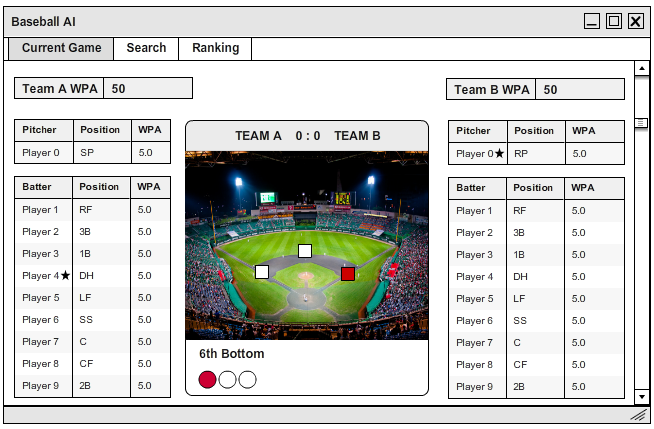
\includegraphics[width=6cm]{Current-game.png}
\caption{Current Game}
\end{figure}

\subsubsection{Player Ranking}
\begin{itemize}
\item Sort players by team, position with WPA stats.
\end{itemize}

\begin{figure}[H]
\centering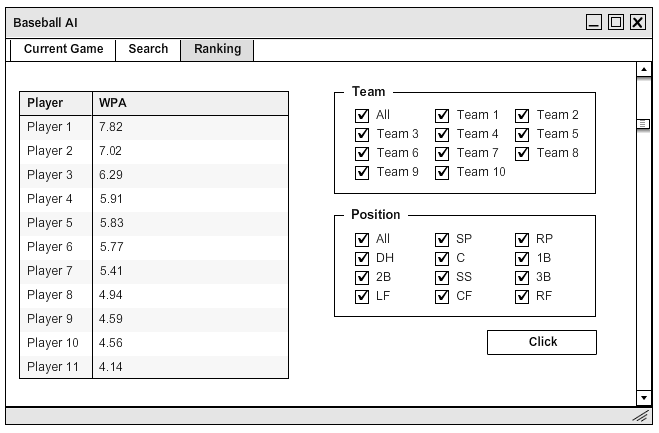
\includegraphics[width=6cm]{Ranking}
\caption{Player Ranking}
\end{figure}

\subsubsection{Data Searching}
\begin{itemize}
\item Search option constitutes of  ‘Search Match/ Search Player’
\end{itemize}
\begin{figure}[H]
\centering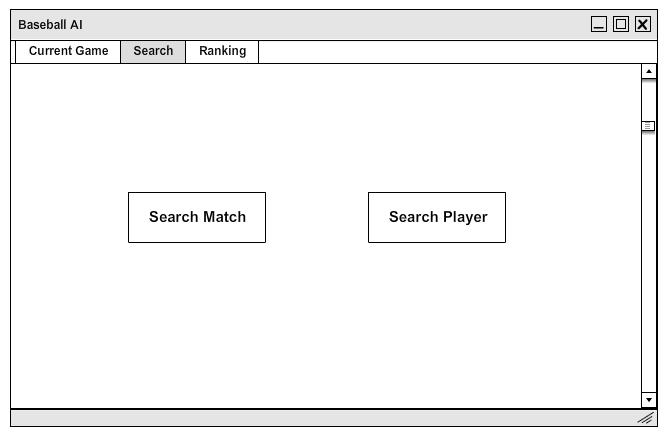
\includegraphics[width=6cm]{Search}
\caption{Search Option}
\end{figure}

\begin{itemize}
\item If option ‘Search Match’ is chosen, program shows match schedule as a calendar.
\end{itemize}
\begin{figure}[H]
\centering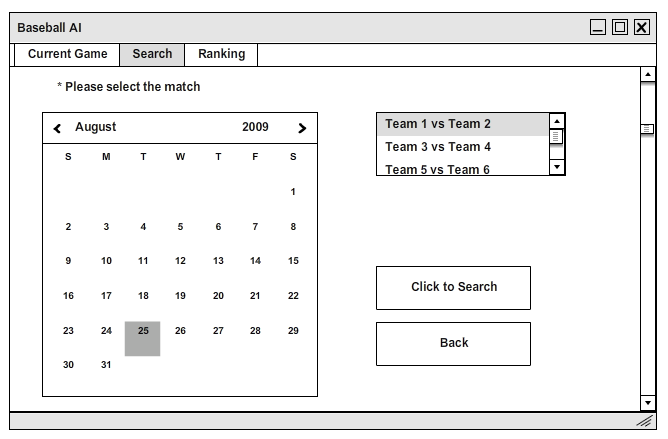
\includegraphics[width=6cm]{Search-match}
\caption{Search-match option}
\end{figure}

\begin{itemize}
\item The result is shown as follows.
\end{itemize}
\begin{figure}[H]
\centering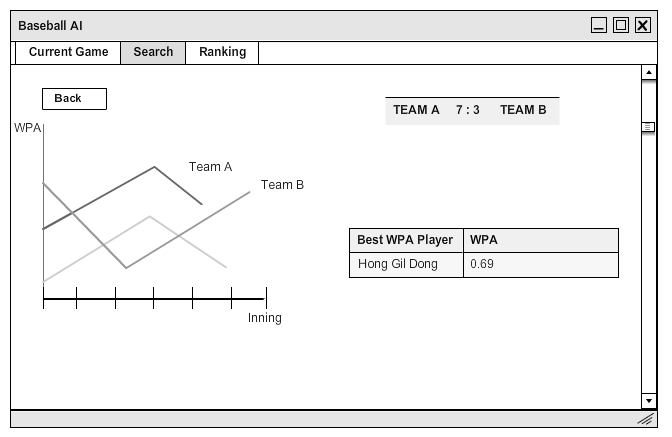
\includegraphics[width=6cm]{Search-match-result}
\caption{Search match result}
\end{figure}

\begin{itemize}
\item If option ‘Search Player’ is chosen, input box will appear. It requires user to enter a player’s name.
\end{itemize}
\begin{figure}[H]
\centering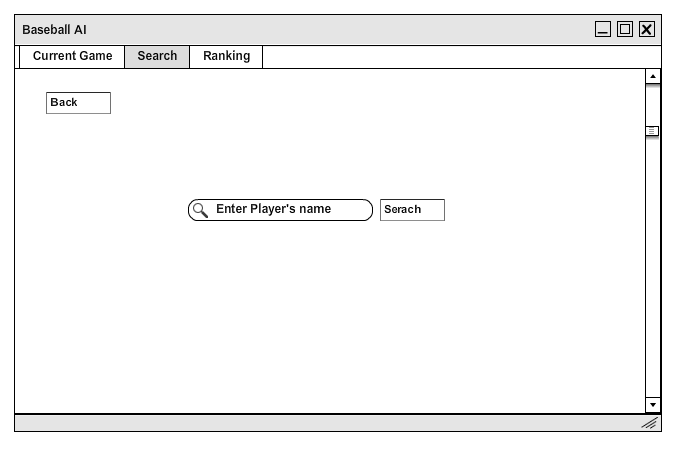
\includegraphics[width=6cm]{Search-player}
\caption{Search Player}
\end{figure}

\begin{itemize}
\item The result is shown as follows.
\end{itemize}
\begin{figure}[H]
\centering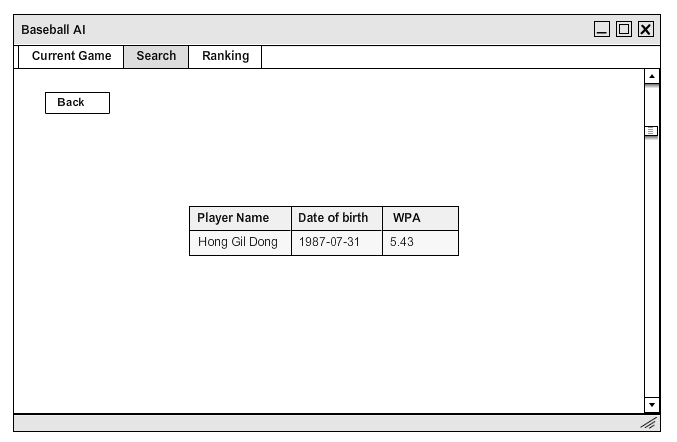
\includegraphics[width=6cm]{Search-player-result}
\caption{Search Player Result}
\end{figure}


\subsubsection{Get Information Real-Time}
\begin{itemize}
\item User can choose the way one gets some information(pop-up or push window).
\item Pop-up is a kind of window, so when user have it on the screen, one cannot click main program.
\item Information could be as follows.
\item Agreed Decision : User can get information about agreed decision and its details.
\item Cancellation in case of rain : User can get information when the match is cancelled in case of rain by getting a pop-up or push window.
\item Player Substitutition : In case of substituting player, User can get information why the player was substituted with other, and information about that ‘other’  player.
\item When option is ‘pop-up’, user can have additional function which is ‘multi-view’.  By doing so, user can watch several matches simultaneously.
\item If there has multiple pop-ups, eliminate pop-up windows sequentially after checking them.
\item Refresh in every 30 seconds.
\end{itemize}



\subsubsection{Error}
\begin{itemize}
\item  If program does not receive signal for 2 minutes, error message pops up with alert sound(windows alert sound).
\end{itemize}
\begin{figure}[H]
\centering\includegraphics[width=6cm]{error1}
\caption{Error Notification}
\end{figure}

\subsubsection{Database}
\begin{itemize}
\item We need four data tables, and each every table refers to each other.
\item We also need one Season table.
\end{itemize}


\begin{figure}[H]
\centering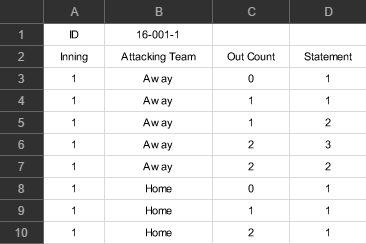
\includegraphics[width=6cm]{match_table_1}
\caption{the first half match table}
\end{figure}

\begin{figure}[H]
\centering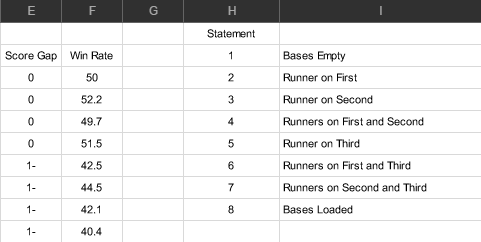
\includegraphics[width=6cm]{match_table_2}
\caption{the second half match table}
\end{figure}

\begin{figure}[H]
\centering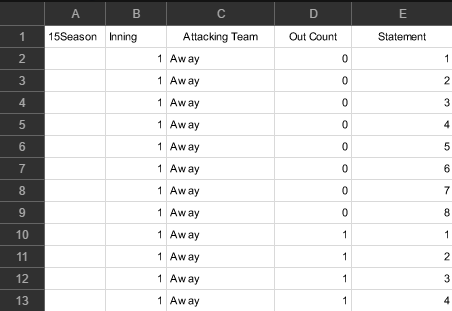
\includegraphics[width=6cm]{sea_state_1}
\caption{the first half season statement table}
\end{figure}

\begin{figure}[H]
\centering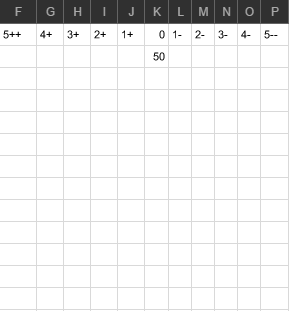
\includegraphics[width=6cm]{sea_state_2}
\caption{the second half season statement table}
\end{figure}

\begin{figure}[H]
\centering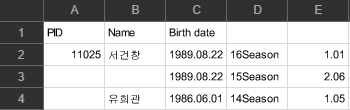
\includegraphics[width=6cm]{player_table}
\caption{player table}
\end{figure}




\section{Architecture Design \& Implementation(partial)}

\subsection{Overall architecture}

\begin{figure}[H]
\centering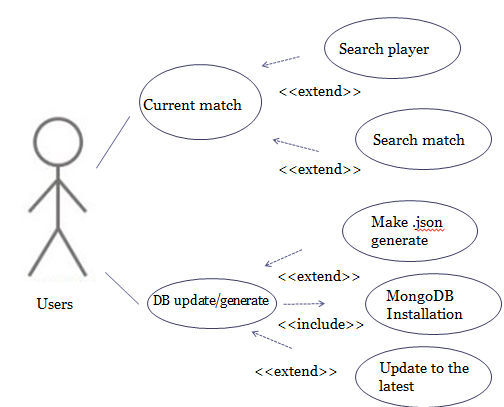
\includegraphics[width=6cm]{Architecture}
\caption{Easy Architecture}
\end{figure}

\begin{figure}[H]
\centering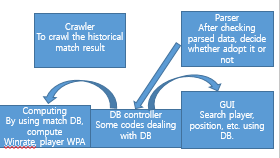
\includegraphics[width=6cm]{ModuleRelation}
\caption{ModuleRelation}
\end{figure}

\begin{itemize}
\item Crawler \\
crawl the historical match result\\
Class1 : pastSpider\\

\item Parser \\
After checking parsed data, decide whether adopt it or not. \\ 
Class1 : game\_checker \\
Class2 : html\_parse \\ 

\item Computing \\
By using match DB, compute Winrate, player WPA.\\
Class1 : make\_winrate\\
Class2 : make\_player\_wpa\\
Class3 : current\_game\\

\item DB controller\\
Some codes dealing with DB\\
Embedded in crawling code. no separate class made.\\

\item GUI
Search player, position, etc. using DB.\\
Class1 : gui\\
Class2 : tabbed\\
Class3 : search\_p\\
Class4 : resultplayerpanel\\
Class5 : search\_m\\
Class6 : dbgen\\
\end{itemize}


\subsection{Directory organization}

\begin{center}
\begin{tabular}{1|1|1|1} \hline
Directory	& File names 				& Module names in use  & Etc.	\\ \hline
./db/     		& match\_log				& computing 		   &		\\ \hline
./db/      		&  player\_wpa			& GUI				   &		\\ \hline
./db/ 		&  winrate				& GUI				   &		\\ \hline
./db/     	  	&  current\_match			& GUI				   &		\\ \hline
./      		&  baseball\_AI			& main module		   &		\\ \hline
\end{tabular}
\end{center}

\subsection{module 1}
Crawling : \\
Crawl raw box data to make past match log. \\
class1 pastSpider : crawl every single KBO website till when DB is made initially. \\
And make match\_log in db updateSpider : crawl KBO website only for needs to be updated.\\
(if last db was ver. 20160528, and today is 20160531, update for 29,30 for automatically)

\subsection{module 2} 
Parsing : \\
Parse the crawled data to make some useful information. \\
class1 game\_checker : parse crawled data to check it is valid website or not. \\ 
class2 html\_parse : after game\_checker adopt specific website, leaving only meaningful values to make DB "match\_log" \\

\subsection{module 3}
Computing : \\  
Compute winrate and WPA from match log, by changing box data to statement data. \\ 
class1 make\_winrate : read box data in "match\_log" and get statement data and save into "winrate" \\  
class2 make\_player\_wpa : read "match\_log" and compute the plus and minus value of winrate and save wpa values into "player\_wpa"\\
class3 current\_game  : using box data crawled by current\_spider make statement data to save into "current\_game"
 

\subsection{module 4}
DB manipulator : \\ 
not decided yet clearly. \\

\subsection{module 5}
GUI : \\
class1 gui : Root frame that all of the contents are integrated.in\\
class2 Tabbed : basic format of panel which is used to declare each tab.in frame.\\
class3 search\_p : action which occurs when ‘Search Player’ button is clicked.\\
class4 resultplayerpanel : panel which pops up to show the result of 'Search Player'\\
class5 search\_m : action which occurs when ‘Search Match’ button is clicked.\\
class6 dbgen : generate or update database when such button is clicked.\\





\section{Use Cases}

\subsection{Current Match}

\begin{figure}[H]
\centering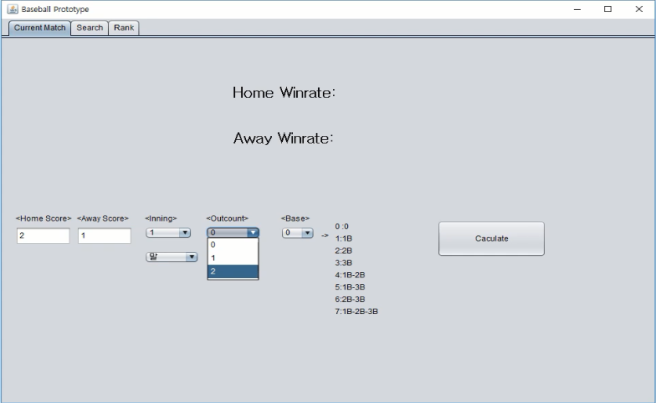
\includegraphics[width=6cm]{WinrateCalculator}
\caption{Winrate calculator based on statement}
\end{figure}

\begin{itemize}
\item You can choose the current situation of the match. Ex) score, inning, outcount, base
\end{itemize}
\begin{itemize}
\item If you finish putting the value and push on the calculate tab, the home winrate and away winrate is calculated and showed on the program.
\item It is based on the latest database you updated or the existing one.
\end{itemize}


\subsection{Player Search}

\begin{itemize}
\begin{figure}[H]
\centering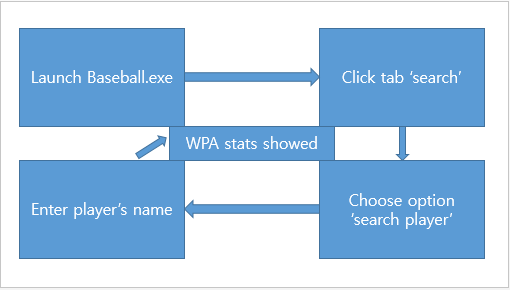
\includegraphics[width=6cm]{PlayerSearch-fc}
\caption{Player Search-flow chart}
\end{figure}
\begin{figure}[H]
\centering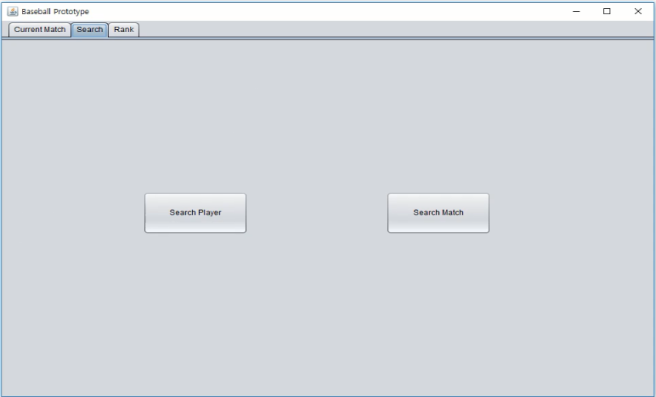
\includegraphics[width=6cm]{SearchButton}
\caption{Search button}
\end{figure}
\item If Users choose the search tap, User can choose between Search Player and Search Match.
\begin{figure}[H]
\centering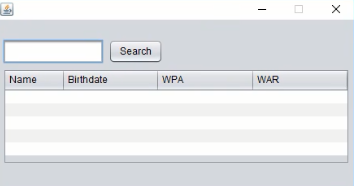
\includegraphics[width=6cm]{PlayerSearch}
\caption{Player search pop-up}
\end{figure}
\begin{figure}[H]
\centering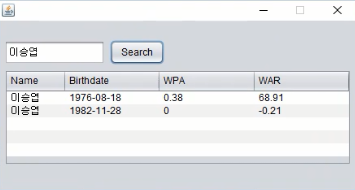
\includegraphics[width=6cm]{PlayerSearchResult}
\caption{Player search result}
\end{figure}
\item If the user clicks on search player tab, another tab is on which users can put the name of the player.
\item If there is many names of the player that have the same name, the all players are shown on the table.
\item The existing information is name, birthdate, WPA, WAR of the player.
\end {itemize}


\subsection{Match Search}

\begin{itemize}
\begin{figure}[H]
\centering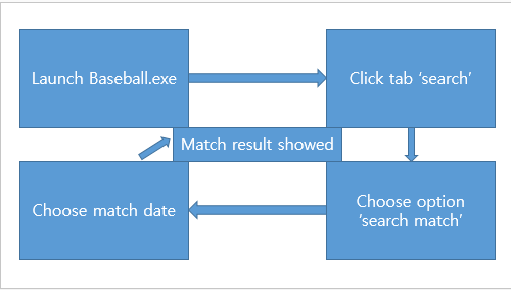
\includegraphics[width=6cm]{MatchSearch-fc}
\caption{Match Search-flow chart}
\end{figure}

\begin{figure}[H]
\centering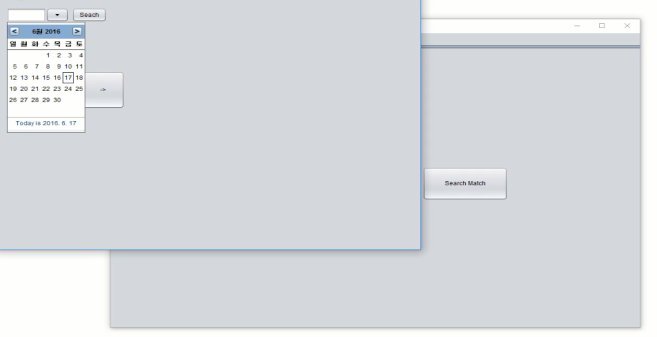
\includegraphics[width=6cm]{MatchSearchDate}
\caption{Match Search\_date choose}
\end{figure}
\item if users click on the ‘search match’ tap, there shows calendar on which you can put the date.
\begin{figure}[H]
\centering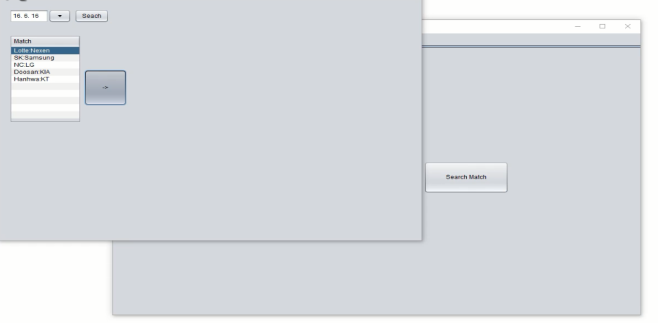
\includegraphics[width=6cm]{MatchSearchMatch}
\caption{Match Search\_match choose}
\end{figure} 
\item After users pick the date, you can get all the list of the matches on that date.

\begin{figure}[H]
\centering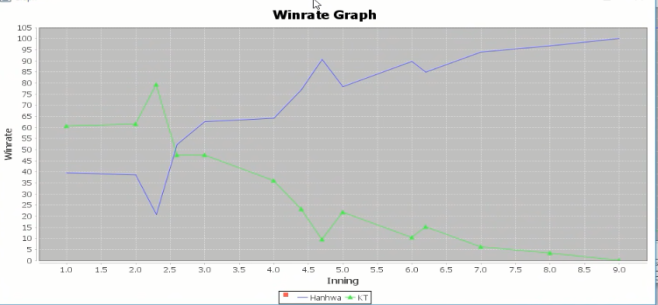
\includegraphics[width=6cm]{MatchSearchGraph}
\caption{Match Search\_Winrate Graph}
\end{figure}
\item The winrate for all innings of each team are shows by linear graph.
\item The values of two graphs are added up to 100\% for every innings. 
\begin{figure}[H]
\centering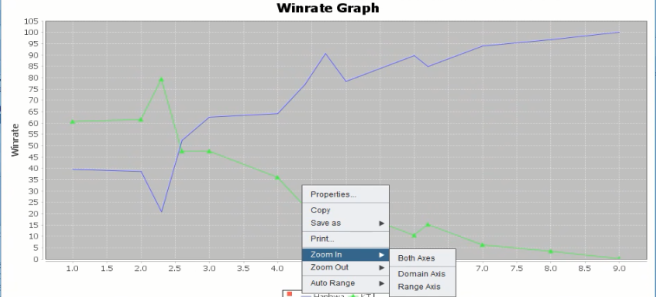
\includegraphics[width=6cm]{MatchSearchGraphZoom}
\caption{Graph option\_zoom in, zoom out}
\end{figure}
\item Users can view the graph in bigger form by clicking on zoom in button, and in smaller form by clicking on zoom out button.
\begin{figure}[H]
\centering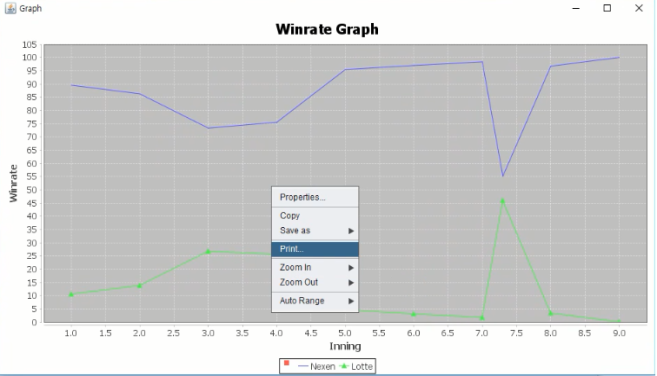
\includegraphics[width=6cm]{MatchSearchGraphPrint}
\caption{Graph option\_print graph}
\end{figure}
\item Users can print the output by clicking on print tab.
\item If users click on it, users can set more details such as size of the sheet, the direction of the print, the margins on the sides,top and bottom.
\begin{figure}[H]
\centering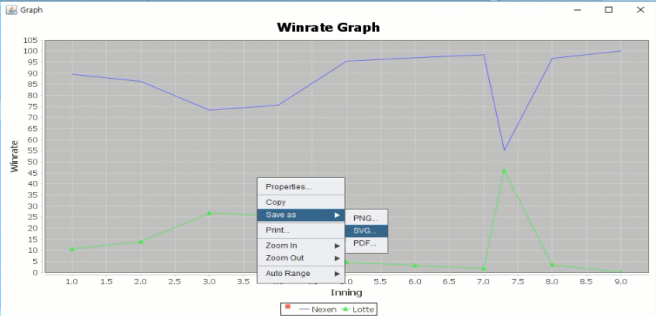
\includegraphics[width=6cm]{MatchSearchGraphSave}
\caption{Graph option\_save graph}
\end{figure}
\item If users click on the save as tab, users can save the graph output by the file form they want.
\item This program supports file form PDF, SVG, and PNG.
\end{itemize}


\subsection{DB generation}

\begin{itemize}
\begin{figure}[H]
\centering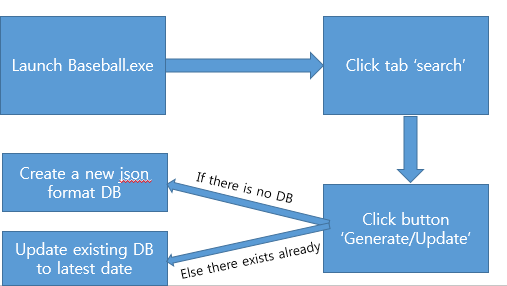
\includegraphics[width=6cm]{DBgeneration-fc}
\caption{DB generation-flow chart}
\end{figure}

\item This program uses MongoDB as data flatforms. By using MongoDB, much of the program functionality can be accessed thorugh JAVA and python.
\begin{figure}[H]
\centering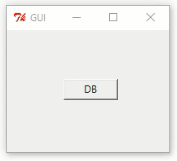
\includegraphics[width=6cm]{DBGeneration}
\caption{DB generating program}
\end{figure}
\item If users click out the GUI.exe, users can generate/update DB
\begin{figure}[H]
\centering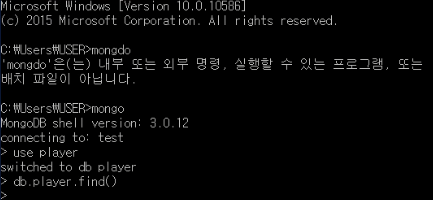
\includegraphics[width=6cm]{BeforeDBGeneration}
\caption{Before\_client DB generation}
\end{figure}
\item Users need to load cmd to generate another DB.
\item Users initially generate/update db my putting the line \'mongo\', \'use player\' and \'db.player.find()\' sequentially.
\begin{figure}[H]
\centering\includegraphics[width=6cm]{AfterDBGeneration}
\caption{After\_client DB generation}
\end{figure}
\item The whole DB is generated or updated with the clicking on the \'DB\' button in \'GUI\' program afer you put the line on the cmd.

\section{Software Installation Guide}

\subsection{MongoDB}
\begin{figure}[H]
\centering\includegraphics[width=6cm]{mongo1}
\caption{MongoDB Logo}
\end{figure}
In order to execute the baseball.ai file, we first need MongoDB. Many exe file don’t need any language program or other platforms because they all aimed to just ‘execute’. However, this baseball.ai file has to be installed to get to the database created by file. MongoDB is a free and open-source cross-platform document-oriented database. It’s classified as a NoSQL database, and it avoids the traditional table-based relational database structure in favor of JSON-like documents with dynamic schemas. With the use of MongoDB, much of the functionality can be accessed through JAVA and python. MongoDB can be used as a file system, taking advantage of load balancing and data replication features over multiple machines for storing files. Files can be distributed and copied multiple times between machines transparently, thus effectively creating a load-balanced and fault-tolerant system. \\
Installation MongoDB on windows.\\

\subsubsection{Step1}
Visit downloads page and find your version of Windows. We are going to place all these files directly inside a directory C:/mongodo/. So once the download finishes, extract the zip and open the folders until you find /bin/ with a few other files. Select all these and cut/paste into our new C:/mongodb/directory.
\begin{figure}[H]
\centering\includegraphics[width=6cm]{mongo2}
\caption{www.mongodb.org/}
\end{figure}
http://www.mongodb.org/ \\
http://www.mongodb.org/downloads\\
\begin{figure}[H]
\centering\includegraphics[width=6cm]{mongo3}
\caption{version/os check}
\end{figure}
Check your version and OS then downloads.\\ \\


\subsubsection{Step2}
Add route. Add new route named MONGODB\_HOME and put the address on which you uncompressed.\\
Revise Path as showed below.
\begin{figure}[H]
\centering\includegraphics[width=6cm]{mongo4}
\caption{system variable editting}
\end{figure}

\subsubsection{Step3}
Now, inside this folder alongside /bin create a new folder named "log" which will store all the MongoDB system logs. We also need to create two external directories for data storage, C:/data/ and C:/data/db.
\begin{figure}[H]
\centering\includegraphics[width=6cm]{mongo5}
\caption{data storage directory}
\end{figure}

\subsubsection{Step4}
After creating new directory, and put ‘mongod’ on the DOS command. Then we can see the server is on like below. 
\begin{figure}[H]
\centering\includegraphics[width=6cm]{mongo6}
\caption{db creation using CMD}
\end{figure}
Then, let’s put new command and put word ‘mongo’’. If you are succeed to follow up to here, you can see the databased to ‘test’ , which means that it’s successfully installed.
\begin{figure}[H]
\centering\includegraphics[width=6cm]{mongo7}
\caption{connect on database 'test'}
\end{figure}

\subsubsection{Step5}
If we open up the command prompt and run cd C:/mongodb/bin, we are looking to start the mongod.exe in shell, but after running this you’ll notice the operation will freeze when listening for connections. Well it’s not actually frozen, we are running Mongo directly through the terminal.\\
So, to start comman Mongo automatically as a Windows Service, first create a log file and configuration for the service. The code below executes creating the log file.
\begin{figure}[H]
\centering\includegraphics[width=6cm]{mongo8}
\caption{creating log file}
\end{figure}
Now run the next two lines in terminal to create the service and get it started.
\begin{figure}[H]
\centering\includegraphics[width=6cm]{mongo9}
\caption{creating service and starts}
\end{figure}
Following line shows all current databases on the server:
\begin{figure}[H]
\centering\includegraphics[width=6cm]{mongo10}
\caption{show database}
\end{figure}


\subsection{BaseballAI.exe}
\subsubsection{Search Player}
\begin{figure}[H]
\centering\includegraphics[width=6cm]{proguidesplayer}
\caption{Search Player}
\end{figure}
You can enter the name of player you want. By doing so, you can get his WPA.

\subsubsection{Search Match}
\begin{figure}[H]
\centering\includegraphics[width=6cm]{proguidesmatch}
\caption{Search Match}
\end{figure}
You can select the date of match, then you can get all the list of the matches on that date.

\subsubsection{Winrate Graph}
\begin{figure}[H]
\centering\includegraphics[width=6cm]{proguidesgraph}
\caption{Winrate Graph}
\end{figure}
The win-rate for all innings of each teams’ are showed in linear graph.


\section{Discussion}
We decided to use python because python is a handy programming language to deal with. Our   
real purpose was to crawl data about korea baseball league, which includes the name(korean). Because python 2.7 doesn't support unicode, at first we didn't know how to handle korean encoding.
But at last, we transfer to python 3.5 and java who is free from unicode problem. During that transition, we had to amend what we had done partly or entirely, and it took a non trivial time to accomplish that. That was our first challenge. Second, about parsing. Because our program uses crawled data from HTML source, it is impossible to avoid parsing problem. The basic principle of parsing is quite simple. But like a many cases, the applicated, nested ones made us feel terrible. Sometimes, it tooks 3 to 4 days to parse one web site. Because both python and parsing is something we had never used before, that may be the reason why we had such a difficulties.
And, about non-technical difficulties. this might be related to technical problem.. Because we all members are technically not proficient, so there was some obstacle when we take about out project, or program. For example, our members was distributed their task one by one. But because computer software is inter-related, there is some time one should know other software's basic things. But in terms of that, we were insufficient. And that makes inter-communication more difficult, slows down the talking. 
Through entire curriculum of our department, this class, firstly and mostly, provide students with practical application of what we learn by doing a project. So except for experienced students who did many project before this class, other class including us must be embrassed. But the more milestone of project we finish, the more we could get relief and we were suprised with ourselves that we could do such a things. Especially we really appreciate you and this class that We improved our practical skill by doing this project.

\end{document}



















